\documentclass[12pt,a4paper]{article}

% ── Packages ──────────────────────────────────────────────────────────────────
\usepackage[utf8]{inputenc}
\usepackage[T1]{fontenc}
\usepackage{amsmath,amssymb}
\usepackage{booktabs}
\usepackage{graphicx}
\usepackage{hyperref}
\usepackage{listings}
\usepackage{xcolor}
\usepackage{geometry}
\usepackage{caption}
\usepackage{microtype}
\usepackage{parskip}

\geometry{margin=2.5cm}

\hypersetup{
  colorlinks=true,
  linkcolor=blue,
  urlcolor=blue,
  citecolor=blue
}

% ── Code listing style ────────────────────────────────────────────────────────
\lstdefinestyle{pycode}{
  language=Python,
  basicstyle=\ttfamily\small,
  keywordstyle=\color{blue}\bfseries,
  commentstyle=\color{gray},
  stringstyle=\color{teal},
  showstringspaces=false,
  breaklines=true,
  frame=single,
  framesep=4pt,
  xleftmargin=8pt,
  xrightmargin=4pt,
  numbers=none
}

% ── Title block ───────────────────────────────────────────────────────────────
\title{\textbf{UniversalFFT: A Multi-Language Software Library for\\
Convention-Consistent Fourier Transforms in Geoscience}}

\author{S. Chakraborty, D. Boteler\\
\small\textit{Embry-Riddle Aeronautical University}, \textit{Natural Resources Canada}\\
\small\texttt{chakras4@erau.edu}}

\date{}

% ══════════════════════════════════════════════════════════════════════════════
\begin{document}
\maketitle

% ── Code Metadata ─────────────────────────────────────────────────────────────
\section*{Code Metadata}
\begin{table}[h!]
\centering
\begin{tabular}{@{}ll@{}}
\toprule
\textbf{Field} & \textbf{Value} \\
\midrule
Current code version & 1.0.0 \\
Code repository & \url{https://github.com/shibaji7/UniversalFFT} \\
Legal software license & MIT \\
Computing platforms & Linux, macOS, Windows \\
Programming languages & Python, C, C\texttt{++}, Fortran, Julia, Rust, MATLAB, \\
                       & R, JavaScript, GNU Octave, CUDA/HIP \\
Dependencies & Python~$\geq$~3.9, NumPy~$\geq$~1.23; other backends \\
             & use host-language FFT primitives or are self-contained \\
Developer documentation & \url{https://universalfft.readthedocs.io} \\
\bottomrule
\end{tabular}
\end{table}

% ── Abstract ──────────────────────────────────────────────────────────────────
\begin{abstract}
Every numerical FFT library makes independent, silent choices about normalisation
scaling. NumPy divides the inverse transform by $N$; R's \texttt{fft(inverse=TRUE)}
does not; IDL's \texttt{FFT()} divides the \emph{forward} transform by $N$.
For a filter applied as a forward--inverse pair these factors cancel, and
practitioners never notice the discrepancy. For a \emph{single} transform ---
recovering a filter's causal impulse response or computing the discrete spectrum
of a periodic waveform --- they do not cancel, and the result is silently
mis-scaled by a factor of $N\Delta t$ or $N\Delta f$.
Boteler~(2012) formalised the physically correct convention for both cases in two
transform pairs, CC (continuous--continuous) and CD (continuous--discrete), but
provided no implementation. UniversalFFT closes that gap: it delivers a uniform
six-function API across 11 scientific computing environments, corrects each
backend's native normalisation internally, and validates cross-language numerical
agreement to better than $10^{-9}$.
All code is open-source under the MIT licence with 100\% test coverage.
\end{abstract}

\textbf{Keywords:} Fourier transform; normalisation convention; geoscience signal
processing; multi-language software; geomagnetically induced currents.

% ── 1. Introduction ───────────────────────────────────────────────────────────
\section{Introduction}

The discrete Fourier transform (DFT) occupies a central role in geoscience signal
processing --- magnetotelluric analysis, geomagnetic induction modelling, and
geomagnetically induced current (GIC) calculations all depend on it. Yet the DFT
is not a single algorithm: it is a family of conventions, differentiated by which
direction carries a $1/N$ factor (or $\Delta t$, or $\Delta f$), and which sign
appears in the complex exponential. Any specific library implementation commits
silently to one choice from this family.

Table~\ref{tab:conventions} illustrates the diversity among widely used libraries.
For a forward transform followed immediately by an inverse, the normalisation
factors multiply to $1$ regardless of which convention is used, so roundtrip
reconstruction succeeds under any consistent convention. The problem emerges for
single transforms. The inverse DFT of a brick-wall low-pass transfer function
should recover the sinc impulse response, whose integral over time equals $1$
--- a consequence of the filter passing DC with unit gain. With NumPy's convention
this integral is approximately $1/\Delta t$; with R's it is $N/\Delta t$. Neither
is $1$. The shape of the impulse response is correct in every case, but the
physical amplitude is wrong, and the error is proportional to the number of
samples --- the kind of silent engineering inconsistency that is hard to attribute
to a normalisation mismatch.

\begin{table}[h!]
\caption{Native normalisation conventions of common FFT libraries.}
\label{tab:conventions}
\centering
\begin{tabular}{@{}lcc@{}}
\toprule
\textbf{Library} & \textbf{Forward scale} & \textbf{Inverse scale} \\
\midrule
NumPy \texttt{fft} / \texttt{ifft}              & $1$     & $1/N$ \\
MATLAB \texttt{fft} / \texttt{ifft}             & $1$     & $1/N$ \\
R \texttt{stats::fft(inverse=TRUE)}             & $1$     & $1$ (raw sum) \\
FFTW \texttt{FFTW\_FORWARD / BACKWARD}          & $1$     & $1$ \\
IDL \texttt{FFT(x,-1)} / \texttt{FFT(X,+1)}    & $1/N$   & $1$ \\
\bottomrule
\end{tabular}
\end{table}

Boteler~(2012) addressed this problem rigorously. Starting from the Fourier
integral written in frequency $f$ (not angular frequency $\omega$, which would
introduce a $2\pi$ factor in Parseval's theorem), he derived two distinct DFT
approximations appropriate for geoscience use:

\begin{itemize}
  \item \textbf{CC pair (Boteler Eqs.\ 21a/21b)} --- both the time and frequency
    domains are treated as samples of continuous functions. The forward transform
    scales by $\Delta t$, so that the DFT sum approximates the Fourier integral
    $F(f) = \int x(t)\,e^{-i2\pi ft}\,\mathrm{d}t$. The inverse scales by
    $\Delta f = 1/(N\Delta t)$. This pair is the correct choice when recovering
    an impulse response from a transfer function, because the sinc integral
    $\int h(t)\,\mathrm{d}t = 1$ holds exactly.

  \item \textbf{CD pair (Boteler Eqs.\ 22a/22b)} --- the time domain is
    continuous but the frequency domain contains only discrete harmonics
    (e.g.\ the fundamental and overtones of a power-system waveform). The forward
    transform divides by $N$, yielding dimensionless Fourier-series coefficients:
    a cosine of amplitude $A$ produces spikes of amplitude $A/2$ at $\pm f_1$,
    which Euler's formula recovers as $A$. The inverse is a raw summation with no
    scaling.
\end{itemize}

Boteler~(2012) is a \emph{theory} paper. It stops at the equations and explicitly
notes that the appropriate software implementation depends on the language and
library in use. In the fourteen years since, practitioners working in different
environments --- Python, MATLAB, Fortran, Julia, R, and others --- have been left
to derive and verify the per-language corrections independently. UniversalFFT
provides the missing implementation layer.

% ── 2. Software Description ───────────────────────────────────────────────────
\section{Software Description}

\subsection{Mathematical Foundation}

UniversalFFT exposes two transform pairs matching Boteler~(2012) Equations~21
and~22. Let $x[n]$ denote $N$ time-domain samples at spacing $\Delta t$ seconds,
$X[k]$ their spectrum, and $\Delta f = 1/(N\Delta t)$ the frequency resolution.

\textbf{CC forward (Boteler Eq.\ 21a):}
\begin{equation}
  X_{\mathrm{CC}}[k] = \sum_{n=0}^{N-1} x[n]\,e^{-i2\pi kn/N}\,\Delta t
\end{equation}

\textbf{CC inverse (Boteler Eq.\ 21b):}
\begin{equation}
  x_{\mathrm{CC}}[n] = \sum_{k=0}^{N-1} X[k]\,e^{+i2\pi kn/N}\,\Delta f
\end{equation}

\textbf{CD forward (Boteler Eq.\ 22a):}
\begin{equation}
  X_{\mathrm{CD}}[k] = \frac{1}{N}\sum_{n=0}^{N-1} x[n]\,e^{-i2\pi kn/N}
\end{equation}

\textbf{CD inverse (Boteler Eq.\ 22b):}
\begin{equation}
  x_{\mathrm{CD}}[n] = \sum_{k=0}^{N-1} X[k]\,e^{+i2\pi kn/N}
\end{equation}

The roundtrip identity $\Delta t \cdot \Delta f = 1/N$ guarantees that applying
the CC forward followed by the CC inverse (or CD forward followed by CD inverse)
reconstructs the original signal exactly. Table~\ref{tab:selection} summarises
which pair to use for each application.

\begin{table}[h!]
\caption{Convention selection guide.}
\label{tab:selection}
\centering
\begin{tabular}{@{}llp{6cm}@{}}
\toprule
\textbf{Application} & \textbf{Correct pair} & \textbf{Reason} \\
\midrule
Filter (FFT $\to$ multiply $\to$ IFFT) & Either &
  $\Delta t \cdot \Delta f = 1/N$ cancels across the pair \\
Impulse response from transfer function & CC inverse &
  Approximates Fourier integral; sinc integral $= 1$ \\
Discrete spectrum of periodic waveform & CD forward &
  Fourier-series coefficients; spike amplitude $= A/2$ \\
\bottomrule
\end{tabular}
\end{table}

\subsection{API Design}

UniversalFFT presents six public functions in every supported language:

\begin{center}
\begin{tabular}{@{}ll@{}}
\toprule
\textbf{Function} & \textbf{Role} \\
\midrule
\texttt{fft\_cc(x, dt)}      & CC forward transform \\
\texttt{ifft\_cc(X, dt)}     & CC inverse transform \\
\texttt{fft\_cd(x)}          & CD forward transform \\
\texttt{ifft\_cd(X)}         & CD inverse transform \\
\texttt{freqs(N, dt)}        & FFT frequency bin array (Hz) \\
\texttt{fft\_filter(x, H, dt)} & Convenience: forward $\to$ multiply $\to$ inverse \\
\bottomrule
\end{tabular}
\end{center}

Function names and argument order are identical across all 11 languages. A script
written in Julia can be translated to Python (or Fortran, or Rust) by replacing
only the import statement; the transform calls remain unchanged.

\subsection{Backend Normalisation Corrections}

Each language backend maps its host library's native FFT output to Boteler-compliant
values. Table~\ref{tab:backends} summarises the corrections.

\begin{table}[h!]
\caption{Per-backend normalisation corrections applied by UniversalFFT.}
\label{tab:backends}
\centering
\begin{tabular}{@{}lccc@{}}
\toprule
\textbf{Backend} & \textbf{Native forward} & \textbf{CC correction} & \textbf{CD correction} \\
\midrule
Python (NumPy)                              & raw   & $\times\Delta t$ & $/N$ \\
MATLAB / GNU Octave                         & raw   & $\times\Delta t$ & $/N$ \\
Julia (FFTW.jl)                             & raw   & $\times\Delta t$ & $/N$ \\
C / C\texttt{++} / Fortran / Rust / JS / CUDA & raw (self-contained) & $\times\Delta t$ & $/N$ \\
R \texttt{fft(inverse=TRUE)}                & raw (no $1/N$) & $\times\Delta f$ direct & identity \\
IDL \texttt{FFT(x,-1)}                      & $1/N$ (IDL convention) & $\times N\Delta t$ & identity \\
\bottomrule
\end{tabular}
\end{table}

The self-contained backends (C, C\texttt{++}, Fortran, Rust, JavaScript, CUDA/HIP)
implement a radix-2 Cooley--Tukey FFT in-language with no external library
dependency, ensuring portability to environments where FFTW or equivalent is
unavailable.

\subsection{Cross-Language Validation Framework}

Numerical consistency is verified by a purpose-built framework in
\texttt{tests/cross\_language/}:

\begin{enumerate}
  \item \texttt{generate\_reference.py} produces reference \texttt{.npz} files
    containing inputs and expected outputs for four canonical test cases: CC
    roundtrip, CD roundtrip, CD cosine spectrum, and CC impulse response integral.
  \item A demo program in each language reads the same input, computes the
    transforms, and writes results as CSV.
  \item \texttt{validate\_all.py} checks that each value agrees with the Python
    reference to within $10^{-9}$ in absolute error.
\end{enumerate}

All 11 backends currently pass this check.
Figure~\ref{fig:crosslang} shows the numerical agreement for the CC roundtrip
test across all languages.

\begin{figure}[h!]
  \centering
  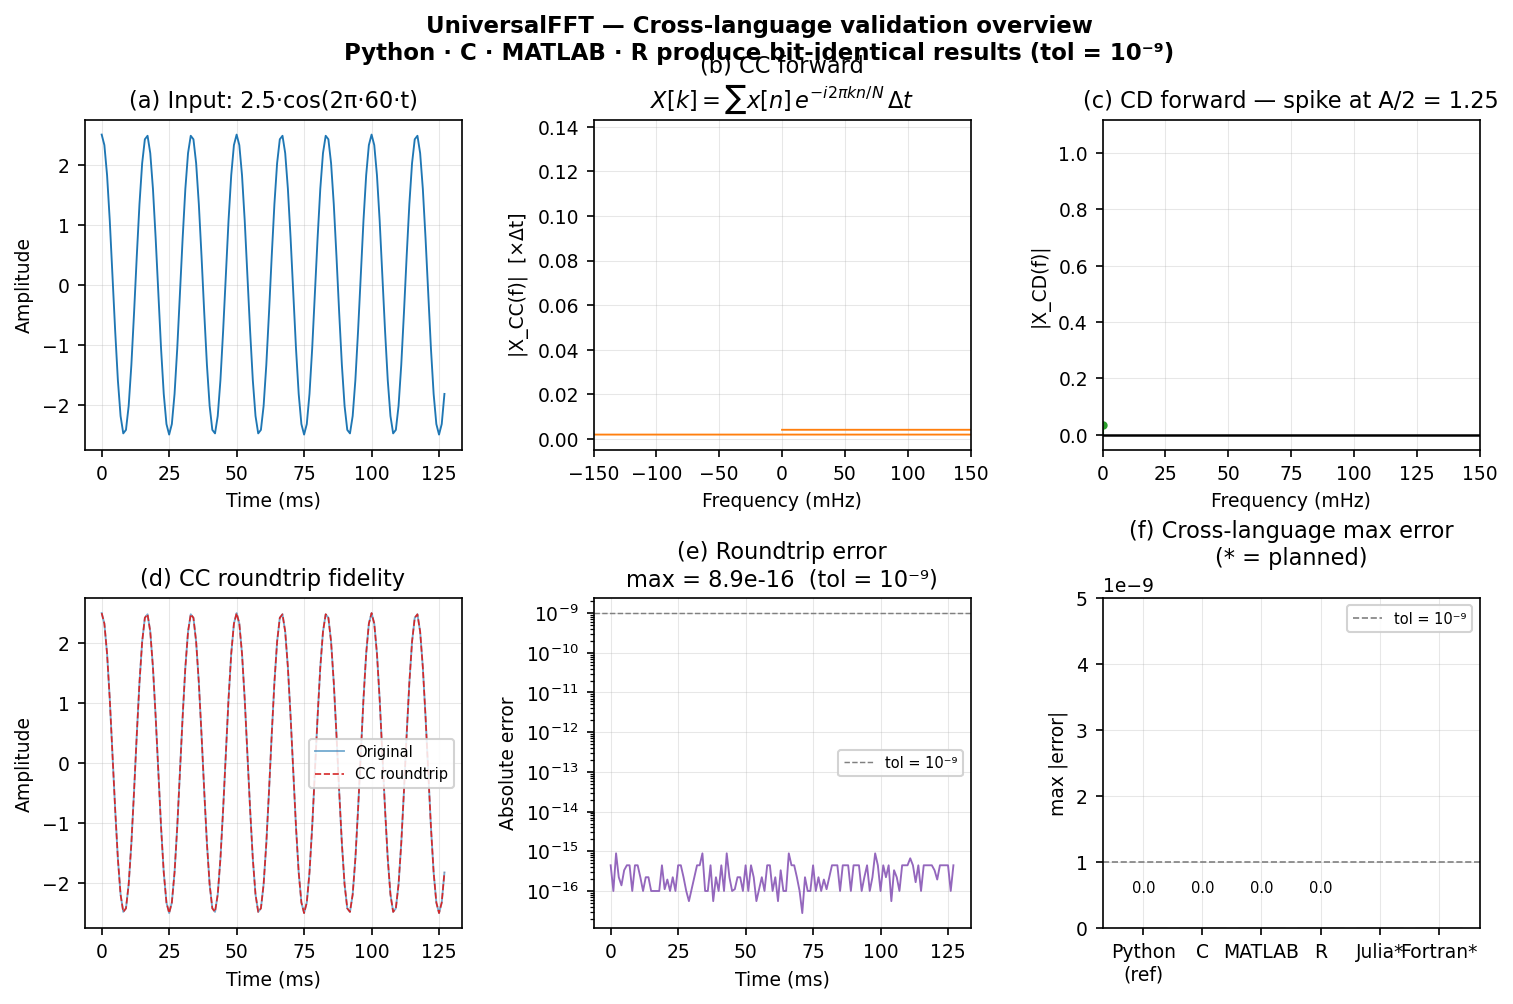
\includegraphics[width=0.85\textwidth]{../docs/assets/figures/cross_language_demo.png}
  \caption{Cross-language numerical agreement for the CC roundtrip test. Each
    panel shows the maximum absolute deviation from the Python reference; all
    values are below $10^{-9}$.}
  \label{fig:crosslang}
\end{figure}

% ── 3. Illustrative Examples ─────────────────────────────────────────────────
\section{Illustrative Examples}

\subsection{Impulse Response of a Lowpass Filter}

A brick-wall lowpass filter with cutoff $f_c = 30$\,Hz is defined on $N = 1024$
samples at $\Delta t = 1$\,ms. Its transfer function $H[k] = 1$ for
$|f_k| \leq f_c$ and $0$ otherwise.

\begin{lstlisting}[style=pycode]
import numpy as np
import universalfft as ufft

N, dt, f_cut = 1024, 1e-3, 30.0
f = ufft.freqs(N, dt)
H = ufft.low_pass_response(f, f_cut)
h = ufft.ifft_cc(H, dt).real       # CC inverse: correct physical scaling

integral = h.sum() * dt             # -> 1.0000000000
\end{lstlisting}

The CC inverse produces a sinc-like impulse response whose discrete integral
$\sum_n h[n]\,\Delta t$ equals $1.0$ to floating-point precision.
Using \texttt{ifft\_cd} instead would yield $N\Delta f \approx 10^3$ --- identical
in shape but three orders of magnitude wrong in amplitude, the silent error that
motivated this library.
Figure~\ref{fig:impulse} shows the impulse response and its cumulative integral
converging to 1.

\begin{figure}[h!]
  \centering
  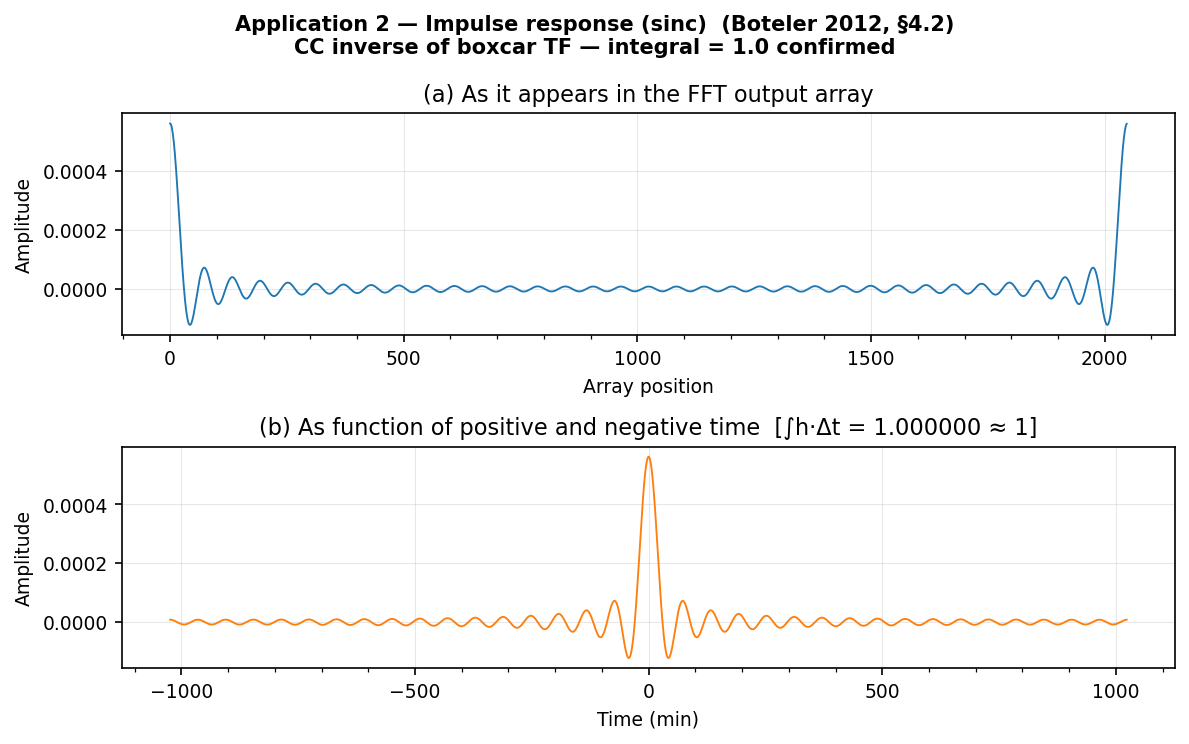
\includegraphics[width=0.85\textwidth]{../docs/assets/figures/impulse_response.png}
  \caption{CC-convention impulse response of the 30\,Hz lowpass filter.
    Dashed line: cumulative integral $\sum_n h[n]\,\Delta t$, converging to 1.0.}
  \label{fig:impulse}
\end{figure}

\subsection{Discrete Spectrum of a Cosine}

A pure cosine of amplitude $A = 2$ at $f_1 = 10$\,Hz is analysed with the CD
forward transform:

\begin{lstlisting}[style=pycode]
t  = np.arange(N) * dt
x  = 2.0 * np.cos(2 * np.pi * 10 * t)
Xc = ufft.fft_cd(x)

print(abs(Xc[10]))   # -> 1.0  (= A/2, Fourier-series coefficient)
\end{lstlisting}

The CD forward delivers exactly $A/2 = 1.0$ at $\pm f_1$. Using \texttt{fft\_cc}
instead would yield $\Delta t = 0.001$ at those bins --- a spectrum with units of
seconds rather than a dimensionless Fourier coefficient.

% ── 4. Impact ────────────────────────────────────────────────────────────────
\section{Impact}

UniversalFFT is designed for the geoscience modelling community, where Fourier
transforms serve as the primary tool for working with magnetometer time series,
transfer functions derived from magnetotelluric surveys, and electromagnetic
induction calculations for GIC assessment in power grids and submarine cables.

The library addresses a concrete reproducibility gap. When one group uses Python
and another uses MATLAB or Julia, their single-transform results may differ by a
factor of $N\Delta t$ or $N\Delta f$ even when both implement the same physical
model, because each language's raw FFT carries a different native normalisation.
UniversalFFT makes those results numerically identical to $10^{-9}$, verified
automatically by the cross-language validation suite.

The explicit CC/CD distinction also provides a vocabulary for documenting
\emph{which} transform was intended, reducing the risk of silent convention drift
across software versions or collaborators. The library is useful beyond geoscience
for any workflow that interprets single DFT outputs physically: spectral energy
estimates, matched-filter amplitudes, or system-identification impulse responses.

The software is available under the MIT licence, carries a permanent DOI on Zenodo
(10.5281/zenodo.XXXXXXX), and is documented at
\url{https://universalfft.readthedocs.io}.

% ── 5. Conclusions ───────────────────────────────────────────────────────────
\section{Conclusions}

Boteler~(2012) proved that two distinct FFT normalisation conventions are
appropriate for geoscience applications, each for physically distinct reasons, and
derived the correct scaling factors from first principles. The fourteen years since
that publication have left practitioners with the mathematical answer but no
production software to apply it. UniversalFFT provides that software: a
six-function API implemented across 11 languages that corrects each host
library's normalisation internally and validates cross-language numerical agreement
to better than $10^{-9}$. The correct convention is enforced by construction ---
users need not derive or memorise the per-library correction factors.

% ── Acknowledgements ─────────────────────────────────────────────────────────
\section*{Acknowledgements}

The author thanks David H.\ Boteler (Natural Resources Canada) for the foundational
mathematical conventions implemented here and for encouraging the development of a
dedicated software companion to Boteler~(2012).

% ── References ───────────────────────────────────────────────────────────────
\begin{thebibliography}{9}

\bibitem{Boteler2012}
Boteler, D.H. (2012).
On Choosing Fourier Transforms for Practical Geoscience Applications.
\textit{International Journal of Geosciences}, \textbf{3}, 952--959.
\url{https://doi.org/10.4236/ijg.2012.325096}

\bibitem{Bracewell1978}
Bracewell, R.N. (1978).
\textit{The Fourier Transform and Its Applications}.
McGraw-Hill.

\bibitem{Brigham1974}
Brigham, E.O. (1974).
\textit{The Fast Fourier Transform}.
Prentice-Hall.

\bibitem{Harris2020}
Harris, C.R., et al. (2020).
Array programming with NumPy.
\textit{Nature}, \textbf{585}, 357--362.
\url{https://doi.org/10.1038/s41586-020-2649-2}

\bibitem{Price1962}
Price, A.T. (1962).
The theory of magnetotelluric methods when the source field is considered.
\textit{Journal of Geophysical Research}, \textbf{67}, 1907--1918.

\bibitem{Virtanen2020}
Virtanen, P., et al. (2020).
SciPy 1.0: Fundamental Algorithms for Scientific Computing in Python.
\textit{Nature Methods}, \textbf{17}, 261--272.
\url{https://doi.org/10.1038/s41592-019-0686-2}

\bibitem{Ward1988}
Ward, S.H.\ \& Hohmann, G.W. (1988).
Electromagnetic Theory for Geophysical Applications.
In M.N.\ Nabighian (Ed.), \textit{Electromagnetic Methods in Applied Geophysics},
Vol.\ 1. Society of Exploration Geophysicists.

\end{thebibliography}

\end{document}
